\documentclass{beamer}
\usepackage[utf8]{inputenc}
\inputencoding{latin1}
\usepackage[T1]{fontenc}
\usepackage[spanish,english]{babel}
\usepackage{graphics}
\usepackage{graphicx}
\usetheme[secheader=true]{Madrid}
\useinnertheme{rectangles}
\usepackage{tikz}
\title{FPGA \& DDR DRAM}
\author[msagre]{Miguel A Sagreras}
\date[2015]{}
%\institution[short name]{long name}
\begin{document}

\begin{frame}
\titlepage
\end{frame}

\section{Primeras computadoras}
\subsection{Tecnolog�a analgica}
\begin{frame}
\frametitle{Torpedo Data Computer}
%\subsection{Electromecánicas Analógicas}
\includegraphics[width=3.2cm]{TDC-image.jpg} 

%\includegraphics[width=3.2cm]{TDC-inside.jpg}
\end{frame}

\subsection{Tecnolog�a digital electromecánica}

\begin{frame}
\frametitle{Relay}
\framesubtitle{Componente básico}
\begin{minipage}[c]{6cm}
	\begin{center}
		\includegraphics[height=3cm]{relay-imagen.jpg}
	\end{center}
\end{minipage}
\begin{minipage}[c]{5cm}
	\begin{center}
		\includegraphics[height=3cm]{relay-diagrama.png}
	\end{center}
\end{minipage}
\end{frame}

\begin{frame}
\frametitle{Z3}
\begin{minipage}[c]{5.25cm}
	\begin{itemize}
		\item A�o 1941
		\item Dise�o Konrad Zuse
		\item Proposito : aeroelasticidad
		\item Palabra de 22 bits
		\item Memoria 64 palabras
		\item Frecuencia alrededor 5 Hz
		\item 2000 relays
		\item 4 KW
		\item Peso 1 Tonelada
	\end{itemize}
\end{minipage}
	\begin{minipage}[c]{6.4cm}
		\includegraphics[width=6.4cm]{Z3_Deutsches_Museum.JPG}
	\end{minipage}
\end{frame}

\subsection{Tecnolgia digital electronica}
\begin{frame}
	\frametitle{Atanasoff-Berry Computer}
	\begin{minipage}[c]{7.5cm}
		\begin{itemize}
			\item Ano 1942
			\item Primera computadora electrocnica 
			\item Resolucion de equaciones diferenciales
			\item Mas de 300 tubos de vacio
			\item 2 DRUM de memoria capacitiva 1600 bits
			\item 30 operaciones por segundo
			\item 320 kg
		\end{itemize}
	\end{minipage}
	\begin{minipage}[c]{4cm}
		\begin{center}
			\includegraphics[width=4cm]{Atanasoff-Berry_Computer_at_Durhum_Center.jpg}
		\end{center}
	\end{minipage}
\end{frame}

\begin{frame}
\frametitle{Memoria Drum}
	\begin{minipage}[b]{7.5cm}
		\begin{itemize}
			\item A�o 1932
			\item Gustav Tauschek
			\item Capacidad de 500 Kbits o 62.5 Kbytes
			\item Precursores de los HDD o discos rigidos
		\end{itemize}
	\end{minipage}
	\begin{minipage}[c]{4cm}
		\begin{center}
			\includegraphics[height=4cm]{Pamiec_bebnowa_1.jpg}
		\end{center}
	\end{minipage}
\end{frame}

\begin{frame}
	\frametitle{Colossus}
	\begin{minipage}[c]{7.5cm}
	\begin{itemize}
		\item Ano 1943-1945
		\item Criptoanalisis
		\item Programacion por interruptores y clavijas
		\item Mas de 1600 tubos de vacio
		\item Apodada Colosus por su tamano.
	\end{itemize}
	\end{minipage}
	\begin{minipage}[c]{4cm}
		\begin{center}
			\includegraphics[width=4cm]{ColossusRebuild_11.jpg}
		\end{center}
	\end{minipage}
\end{frame}

\begin{frame}
\frametitle{ENIAC o Electronic Numerical Integrator And Computer}
\framesubtitle{Descripci�n}
\begin{itemize}
	\item Ano 1943
	\item Proposito : calculo de trayectoria de misiles
	\item Programacion por interruptores y clavijas
	\item $10^{3}$ mas rapida en procesamiento que las electromecanicas
	\item Memoria : 100 palabras de 10 digitos decimales o 4100 bits
	\item Recursos :
		\begin{itemize}
			\small
			\item 17.000 tubos de vacio
			\item 7.200 diodos de cristal
			\item 70.000 resistencias
			\item 10.000 capacitores
			\item 5.000.000 de soldaduras
			\item 150 KW
			\item 167 $m^{2}$
			\item 500.000 USD o 6.000.000 USD actualizados
		\end{itemize}
	\end{itemize}
\end{frame}

\begin{frame}
\frametitle{ENIAC o Electronic Numerical Integrator And Computer}
\begin{center}
	\includegraphics[width=11cm]{ENIAC.png}
\end{center}
\end{frame}

\begin{frame}
\frametitle{UNIVAC I (UNIVersal Automatic Computer I}
	\begin{itemize}
		\item 1951-1954
		\item Proposito comercial
		\item Programaci�n en memoria
		\item Procesamiento : 1.900 operaciones por segundo
		\item Memoria : 1000 palabras de 11 digitos decimales
		\item Recursos :
			\begin{itemize}
				\item 5.200 Tubos de vacio.
				\item Tecnología de memoria Linea de Retardo de mercurio.
				\item 125 KW
				\item 13 toneladas
				\item 35.5 $m^{2}$
				\item Precio original 159.000 incrementandose hasta 1.500.000 USD
			\end{itemize}
	\end{itemize}
\end{frame}

\begin{frame}
	\frametitle{UNIVAC I (UNIVersal Automatic Computer I}
	\begin{center}
		\includegraphics[width=11cm]{UNIVAC-I-BRL61-0977.jpg}
	\end{center}
\end{frame}

\begin{frame}
\frametitle{Memoria de linea de retardo}
\begin{minipage}[c]{7.5cm}
	\begin{itemize}
		\item 1947
		\item John Adam Presper Eckert
		\item Origen en las lineas de retardo para Radar
		\item EDVAC, UNIVAC I
		\item Medio de propagacion Mercurio
	\end{itemize}
\end{minipage}
\begin{minipage}[c]{4cm}
	\begin{center}
		\includegraphics[width=4cm]{delay_line.png}
	\end{center}
\end{minipage}
\end{frame}

\subsection{Transistores}
\begin{frame}
	\begin{itemize}
		\item 1953, Universidad de Manchester, 92 transistores, 550 diodos, 48 bits, 150 Watts
		\item 1954, Bell Laboratories
		\item 1957 IBM 608
	\end{itemize}
\end{frame}

\begin{frame}
\frametitle{Compiladores}
	\begin{itemize}
		\item Principios de los 50s
		\item Programa generador automatico de codigo de maquina
		\item Ejemplos
			\begin{itemize}
				\item Autocode (principios de 1950)
				\item FLOW-MATIC (1955)
				\item FORTRAN (mediados de 1950)
				\item COBOL (1959)
				\item ALGOL
			\end{itemize}
	\end{itemize}
\end{frame}

\begin{frame}
\frametitle{Core memory}
	\begin{minipage}[c]{7.5cm}
		\begin{itemize}
			\item 1955-1975
			\item Toroides m�gneticos
			\item Lectura destructiva
			\item Costo de 1.00(1955) a 0.01(1975) USD por bit
			\item Desplaza a las tecnología de memorias :
				\begin{itemize}
				\item DRUM
					\item Tubos de Vacio
					\item Transistores
				\end{itemize}
			\item Fabricadas por sastres en el este asiatico
		\end{itemize}
	\end{minipage}
	\begin{minipage}[c]{4cm}
		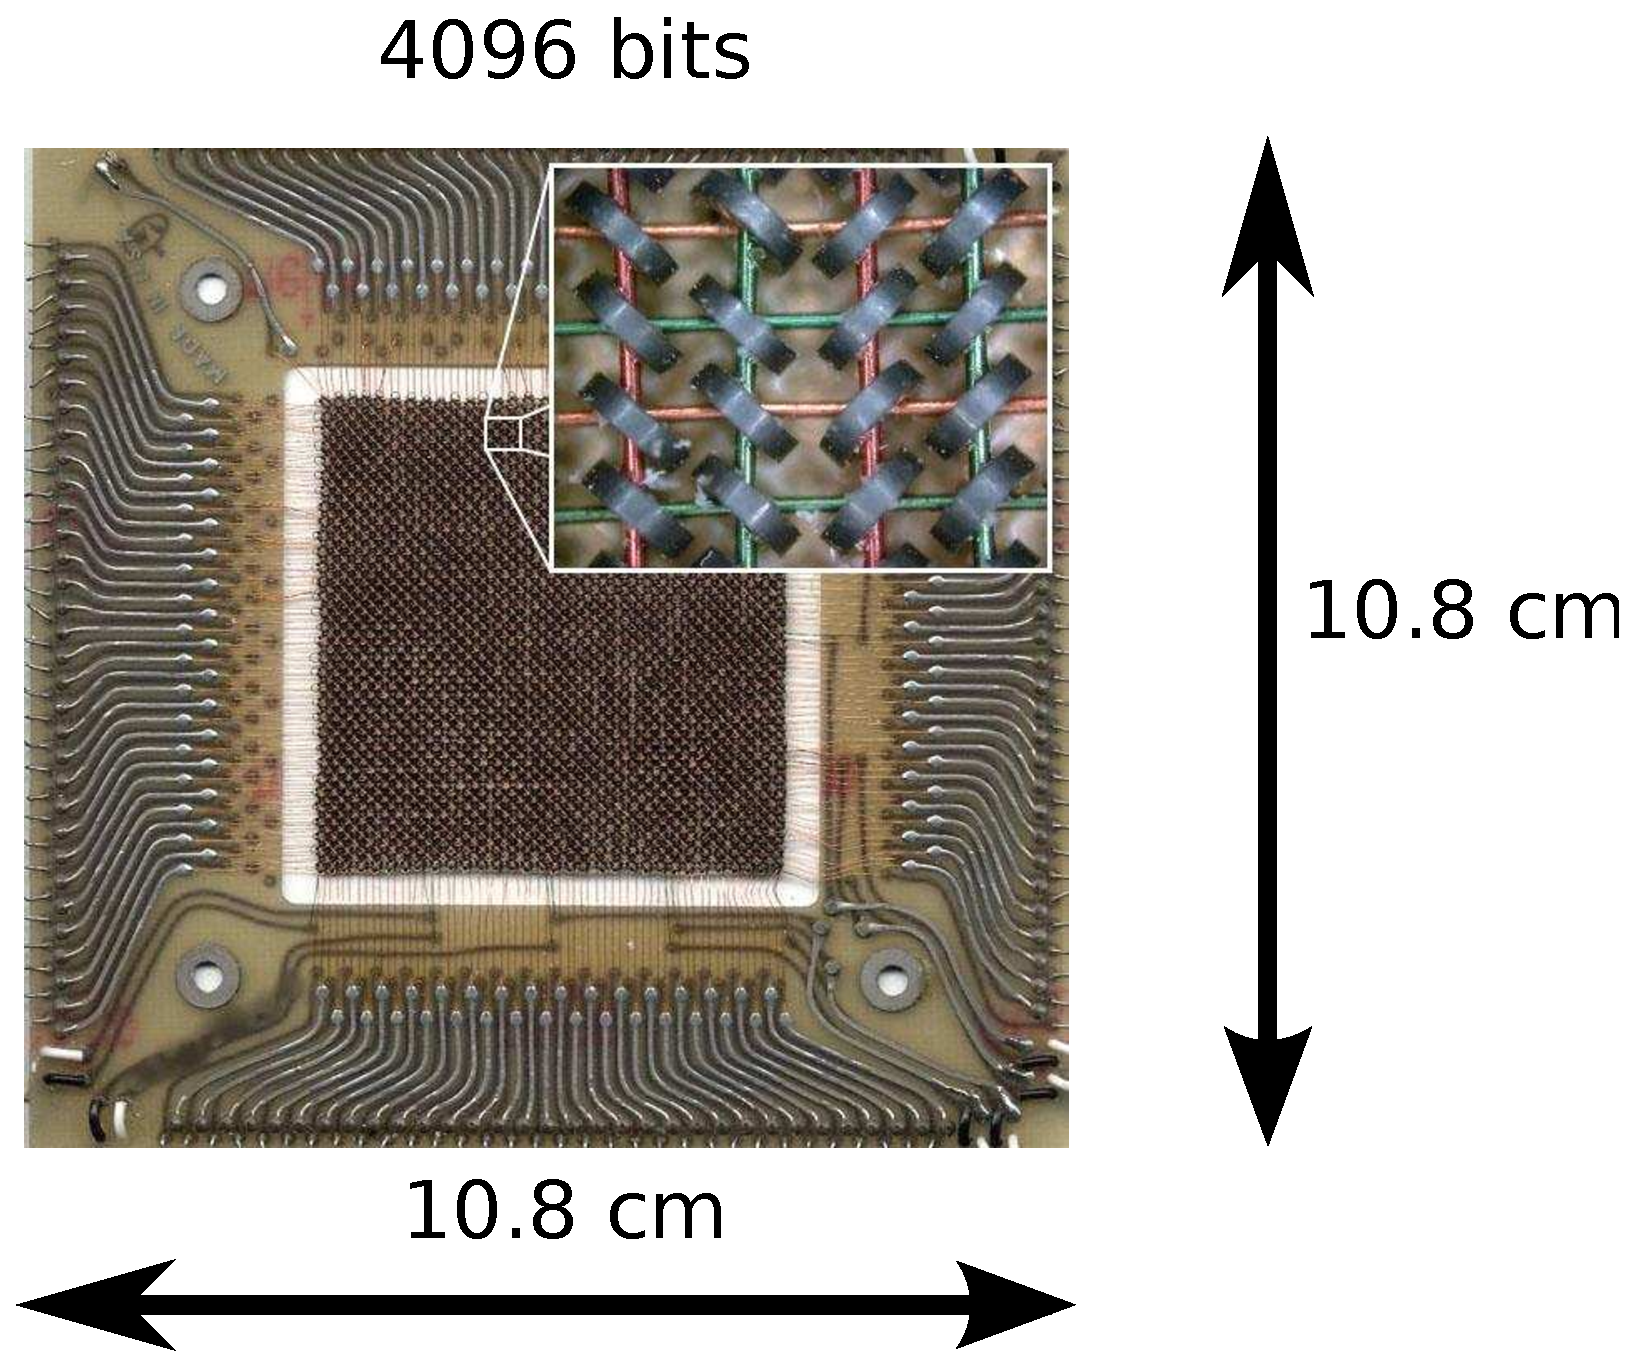
\includegraphics[width=4cm]{Ferrite_core_memory.eps} \\ \\
		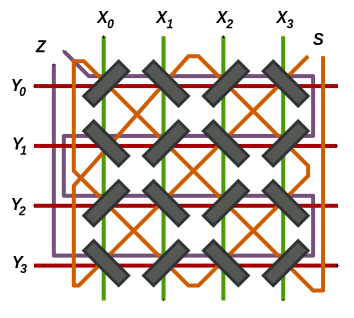
\includegraphics[width=2.5cm]{Coincident-current_magnetic_core.eps}
	\end{minipage}
\end{frame}

\begin{frame}
\frametitle{DRAM Memoria dinámica}
	\begin{minipage}[c]{4.5cm}
		\begin{center}
			\begin{itemize}
				\item Año 1966
				\item Robert Dennard
				\item Un transistor por bit
			\end{itemize}
		\end{center}
	\end{minipage}
	\begin{minipage}[c]{6.5cm}
		\begin{center}
		\includegraphics[width=6.5cm]{onetransistor.png} 
			%	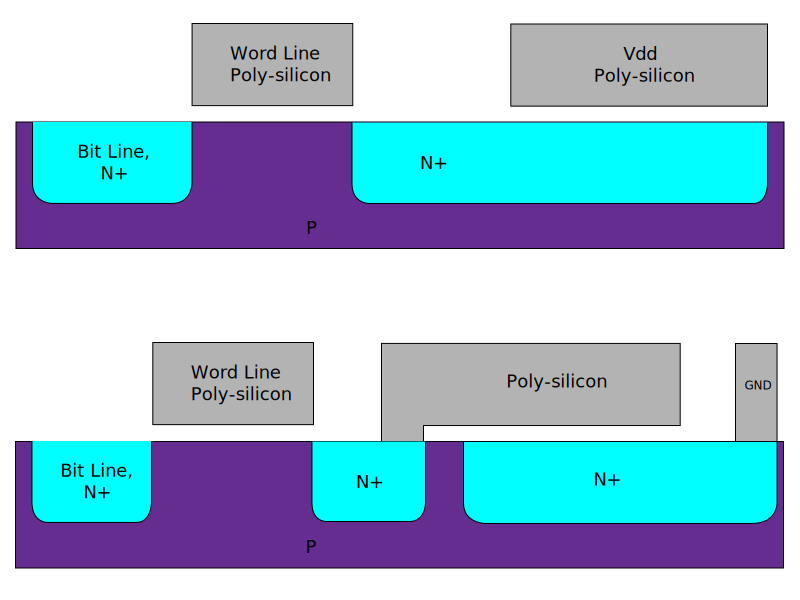
\includegraphics[width=5cm]{Original_1T1C_DRAM_design.eps}
		\end{center}
	\end{minipage}
\end{frame}

\subsection{DRAM}
\begin{frame}
\frametitle{Banco de Memoria}
	\begin{center}
		\includegraphics[width=9cm]{membank.eps}
	\end{center}
\end{frame}

\begin{frame}
\frametitle{Multiplexado de la direccion}
	\begin{itemize}
		\item 1966
		\item Robert Proebsting cofundador de Mostek
		\item Divide la direccion en dos y multiplexa las partes
			\begin{itemize}
				\item Filas \textbf{Row}
				\item Columnas \textbf{Column}
			\end{itemize}
		\item Reduce el tamano del Chip y por consiguiente su costo.
		\item Fue ridiculizado por sus competidores.
		\item A finales del 70s dominaba el 85\% del mercado mundial.
	\end{itemize}
\end{frame}

\begin{frame}
\frametitle{Ley de Moore}
	\begin{itemize}
		\item 1975
		\item Gordon E. Moore
	\end{itemize}
\end{frame}

\begin{frame}
\frametitle{Lenguajes descriptores de hardware}
	\begin{itemize}
		\item Finales de los 60s
		\item Transferencia de Registros
	\end{itemize}
\end{frame}

\begin{frame}
\frametitle{Diagrama en Bloques}
	\begin{center}
		\includegraphics[width=10cm]{chip.eps}
	\end{center}
\end{frame}

\begin{frame}
\frametitle{Secuencia de acceso}
	\begin{itemize}
		\item Acceder a la fila con las lineas precargardas
		\item Conectar el amplificador de sensado
		\item Acceder a la columna
		\item Recuperar el valor leido
		\item Percargar las lineas a la mitad de la tension entre el 0 y el 1 logico
	\end{itemize}
\end{frame}

\subsection{Diagrama de tiempos}
\begin{frame}
	\begin{center}
		\includegraphics[width=11cm]{dram-timings.eps}
	\end{center}
\end{frame}

\begin{frame}
	\begin{center}
		\includegraphics[width=11cm]{sdrdram-timings.eps}
	\end{center}
\end{frame}

\begin{frame}
	\begin{center}
		\includegraphics[width=11cm]{ddrdram-timings.eps}
	\end{center}
\end{frame}

\section{fpga}
\begin{frame}
	\begin{center}
		\includegraphics[width=11cm]{fpga.eps}
	\end{center}
\end{frame}

\end{document}

